\documentclass[a4paper, 12pt, oneside]{book}

\usepackage[utf8]{inputenc}
\usepackage{lmodern}
\usepackage{layout}
\usepackage{emptypage}
\usepackage{fancyhdr}
%\usepackage[spanish,es-tabla]{babel}
\usepackage{cite}
%\usepackage[Conny]{fncychap}
%\usepackage{graphicx}
%\usepackage{subfigure} % subfiguras
\usepackage{caption}
\usepackage{mathtools}
\usepackage{hyperref}
\usepackage[all]{xy}
%\usepackage[a4paper,top=3cm, bottom=3cm, inner=2.5cm, outer=2.5cm]{geometry}


\usepackage[%
    left=1.2in,%
    right=1.2in,%
    top=1.7in,%
    bottom=1.5in,%
    paperheight=11in,%
    paperwidth=8.5in%
]{geometry}

\usepackage{listings}
\usepackage[spanish]{babel}
\usepackage{url}
\usepackage{float}
\usepackage{multirow}
\usepackage{rotating} 
\usepackage{color}
\usepackage{colortbl}
\usepackage[table]{xcolor}
\usepackage[spanish]{babel}
\usepackage{enumerate}
\usepackage{subfig}

\usepackage{afterpage}

\usepackage[acronym, nonumberlist]{glossaries}
\lstset{escapeinside={<@}{@>}}


\makeglossaries

\makeatletter
\renewcommand{\@makeschapterhead}[1]{%
%  \vspace*{50\p@}%
  \vspace*{0\p@}%
  {\parindent \z@ \raggedright
    \normalfont
    \interlinepenalty\@M
    \Huge \bfseries  #1\par \nobreak
%    \vskip 40\p@
    \vskip 15\p@
  }}
\makeatother

\renewcommand{\baselinestretch}{1.4}
\setlength{\headheight}{16pt} 
\captionsetup{justification=justified}
\pretolerance=1000

\chead[]{}
\rhead[]{}
\renewcommand{\headrulewidth}{0.5pt}

\pagestyle{empty}

\title{Despegue, b\'usqueda y aterrizaje}
\author{Jorge Vela Peña}

\renewcommand{\listfigurename}{LISTA DE FIGURAS}
\renewcommand{\chaptername}{Cap\'itulo}
\renewcommand{\contentsname}{\'Indice general}
\renewcommand{\figurename}{Figura}
\lstset{
	float=hbp,
	basicstyle=\ttfamily\small,
	columns=flexible,
	tabsize=4,
	frame=single,
	extendedchars=true,
	showspaces=false,
	showstringspaces=false,
	numbers=none,
	numberstyle=\tiny,
	breaklines=false,
	breakautoindent=true,
	captionpos=b
}
\setcounter{tocdepth}{4}
\setcounter{secnumdepth}{4}

\definecolor{lightgray}{gray}{0.9}

\begin{document}
\begin{titlepage}
	\begin{center}
		\vspace*{3mm}
		\begin{center}
			
\includegraphics[width=0.4\linewidth]{imgs/logo.jpg}
		\end{center}
		\vspace{6.5mm}
		
		\fontsize{15.5}{14}\selectfont ESCUELA TÉCNICA SUPERIOR DE INGENIERÍA INFORMÁTICA
		\vspace{8mm}
		
		\fontsize{14}{14}\selectfont MÁSTER OFICIAL EN VISIÓN ARTIFICIAL
		
		\vspace{60pt}
		
		\fontfamily{lmss}\fontsize{15.7}{14}\selectfont \textbf{TRABAJO FIN DE MASTER} 
		
		\vspace{20mm}
		\begin{huge}
			""DETECTOR BADACOST EN C++""
		\end{huge}
		
		\vspace{20mm}
		
		\begin{large}
			Autor: Jorge Vela Peña
			
			Tutor: José Miguel Buenaposada Biencinto
			
			\vspace{7mm}
		\end{large}
		\begin{normalsize}
			Curso académico 2019/2020		
		\end{normalsize}
		\vspace{7mm}
		
	\end{center}


\end{titlepage}




\clearpage\null\newpage

\pagenumbering{Roman}
\chapter*{Resumen}



\cleardoublepage



%%%%%%%%%%%%%%% Índices %%%%%%%%%%%%%%%%%%%%
%\cleardoublepage
\renewcommand{\tablename}{Tabla}
%\renewcommand{\listtablename}{Índice de tablas}
%\tableofcontents

%\cleardoublepage % Í­ndice de figuras
%\addcontentsline{toc}{chapter}{\listfigurename}
%\listoffigures

%\cleardoublepage % Í­ndice de tablas
%\addcontentsline{toc}{chapter}{Índice de tablas}
%\listoftables 
\cleardoublepage
\tableofcontents % indice de contenidos

\cleardoublepage
\listoffigures % indice de figuras
\addcontentsline{toc}{chapter}{Índice de figuras} % para que aparezca en el indice de contenidos

\cleardoublepage
%\listoftables % indice de tablas
%\addcontentsline{toc}{chapter}{Índice de tablas} % para que aparezca en el indice de contenidos



\pagestyle{fancy}
\pagenumbering{arabic}
\setlength{\parindent}{6mm}

\lhead[]{CAPÍTULO \thechapter. INTRODUCCIÓN}
\chapter{Introducci\'on}\label{cap.introduccion}
\hspace{1 cm} Como parte de la visión artificial, se considera muy importante la detección de objetos en las imágenes. La detección se basa en encontrar elementos determinados en una imagen partiendo de su apariencia visual. Para conseguir esto, se parte de la búsqueda de patrones determinados que definan el elemento a encontrar. Para realizar esta detección, se emplean algoritmos de clasificación, los cuales realizan transformaciones sobre imágenes, intentando obtener esas características determinadas para localizar en que parte se encuentra un elemento de interés (coches o caras, por ejemplo).

A lo largo de este capítulo se va a realizar una introducción sobre los clasificadores, los distintos tipos de clasificadores que existen. Tras ello hablar de varias formas que hay de trabajar con ellos para terminar hablando de un método específico de trabajo, entrando así en el contexto mas cercano de este trabajo.

 
\section{Tipos de clasificadores}

Dentro de los clasificadores, podemos encontrar dos grandes divisiones. Por un lado están los clasificadores débiles, los cuales son ligeramente mejores que los clasificadores aleatorios. Estos clasificadores tienen pocos datos para determinar la clase correcta, siendo adecuados cuando solo existen dos clases. Su error, siendo gamma la ventaja obtenida sobre la aleatoriedad, es \varepsilon = 0.5 - \gamma . 

Por otro lado, un clasificador fuerte es aquel que está bien correlacionado con la clasificación verdadera.

\subsection{Clasificadores débiles}
En esta sección se explican diferentes tipos de clasificadores de esta clase, su funcionamiento y un ejemplo de como trabajan.

\textbf{K-Nearest Neighbor:} Este método busca las observaciones mas cercanas a la que se intenta predecir, y en función de estos datos clasifica el de interés como la mayoría de su alrededor. 
Para su funcionamiento, memoriza los datos del entrenamiento, los cuales utiliza para realizar la predicción. Por ello, se trata de un método de aprendizaje supervisado ya que necesita un conjunto de entrenamiento previamente etiquetado. 

En el siguiente ejemplo, este método trata de clasificar el circulo verde. Para ello, en caso de que tomemos k = 3, siendo k el número de vecinos, se obtendría que el circulo verde es un triangulo. Sin embargo, si tomáramos k = 5, se trataría de un cuadrado azul ya que serían la mayoría de elementos cercanos.

\begin{figure}[ht]
	\centering
		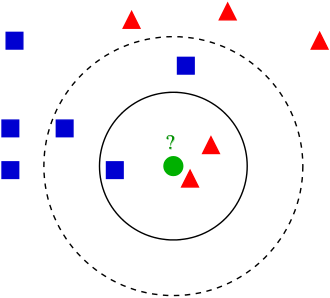
\includegraphics[width=0.3\textwidth]{imgs/knn.png}
		\caption{Ejemplo gráfico KNN.}
	\label{fig:Ejemplo gráfico KNN}
\end{figure}


\textbf{Support Vetor Machine:} Se trata de un clasificador discriminativo el cual busca aprender la frontera entre distintas clases. Cuando se trata de n-dimensiones, el clasificador va a buscar el hiperplano que une a las variables de predicción para crear el limite entre categorías. Este hiperplano va intentar tener la máxima distancia con los puntos que estén alrededor de el, obteniendo así un margen entre las clases. 

En un clasificador de este tipo, no es posible una separación ideal entre clases, por lo que siempre van a surgir errores en la clasificación. En caso de tener un modelo perfecto que no se pueda generalizar para otro conjunto de datos, se produce lo conocido como sobreajuste. 

En la siguiente figura se pueden observar distintos tipos de fronteras entre clases. H1 se trata de una frontera que no hace bien la separación entre clases. H2 es una frontera que hace bien la separación, pero no deja los márgenes óptimos. Sin embargo, H3 realiza una separación correcta entre clases, dejando margenes de distancia con los elementos mas cercanos.

\begin{figure}[ht]
	\centering
		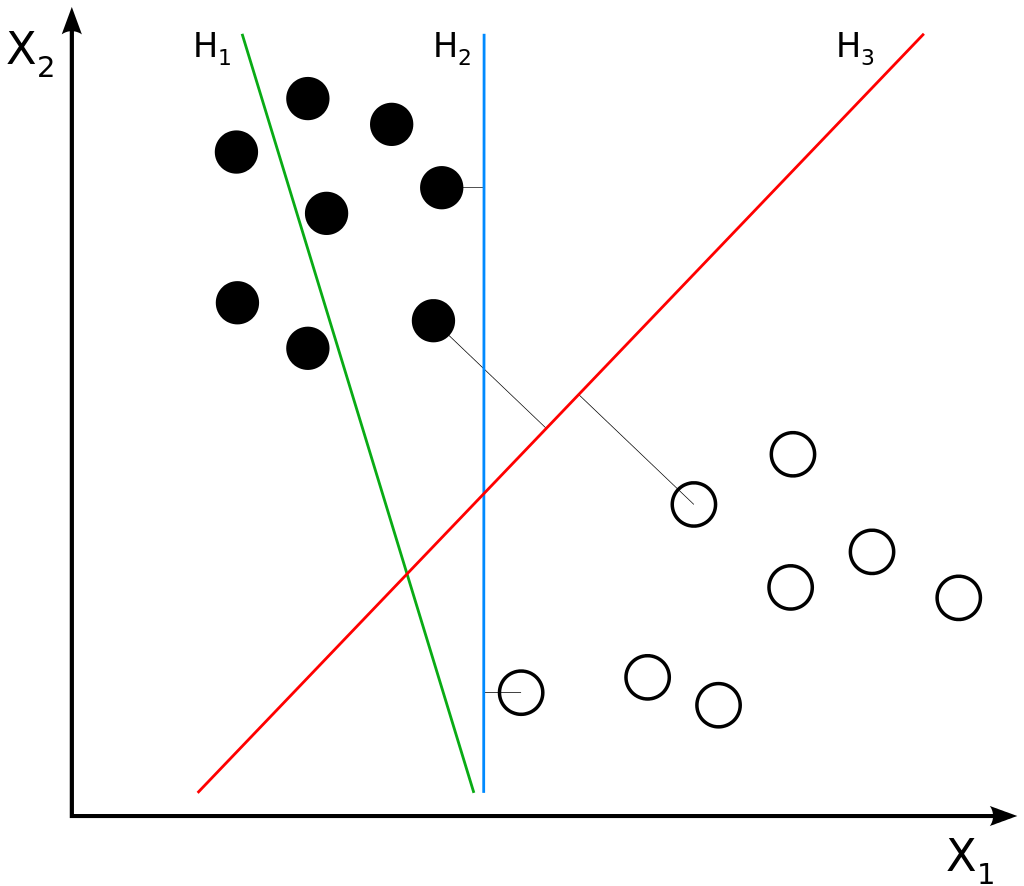
\includegraphics[width=0.3\textwidth]{imgs/SVM.png}
		\caption{Diferentes hiperplanos posibles con SVM.}
	\label{fig:hiperplanos posibles con SVM}
\end{figure}



\subsection{Clasificadores fuertes}
En esta sección se explican distintos clasificadores de este tipo y su funcionamiento.

\textbf{Naive Bayes:} Se trata de un clasificador probabilístico basado en el teorema de Bayes, el cual supone que los atributos de la clase son condicionalmente independientes. Este clasificador trabaja realizando el máximo a posteriori, y pese a que la superposición anterior no es valida para muchos casos, ya que en muchas ocasiones los atributos de las clases son dependientes entre si, Naive Bayes obtiene resultados muy buenos con un coste computacional reducido.
Este tipo de algoritmos son útiles para los casos de multi clases. 


\textbf{Redes de convolución neuronal:} Es un algoritmo de aprendizaje profundo. Estas obtienen una imagen de entrada, las cuales procesa para poder identificar objetos, por ejemplo. Este tipo de algoritmos buscan solos las características deseadas, por ello se necesitan muchas imágenes de un mismo elemento, para que la red pueda obtener esas características comunes.

Existen distintas arquitecturas para este tipo de algoritmos. En la mayoría de casos los modelos de retroalimentación ofrecen resultados muy precisos, especialmente en trabajos con imagen.
Estas arquitecturas pueden tener distintos niveles de capas. Una red debe tener al menos tres capas, una capa de entrada, encargada de recibir datos , una capa oculta, encargada de procesar la información y obtener los datos de interés, y una capa de salida, encargada de retornar la salida de la red. Se puede dar el caso en el que existan varias capas ocultas, haciendo el sistema más complejo, pero también se necesita mas tiempo para entrenamiento. 

En el caso de un sistema complejo con varias capas, las primeras capas son las encargadas de detectar elementos simples (lineas rectas y curvas), para poco a poco especializarse en formas específicas, llegando a reconocer caras y coches, por ejemplo.


\section{Combinación de clasificadores}
En determinadas ocasiones, para realizar un clasificador complejo se hace una combinación de clasificadores. Esto tiene objetivo mejorar un clasificador combinándolo con los demás.
Para realizar la combinación de clasificadores existen diferentes razones. 

\textbf{Razón estadística: } Uno puede encontrarse con conjuntos de datos pequeños en comparación con el tamaño de la hipótesis. Para ello, el método de clasificación puede tener múltiples hipótesis que tengan una precisión similar en el conjunto de datos disponible. Si se combinan diferentes hipótesis, al realizar un promedio de los resultados se reduce el riesgo de seleccionar un clasificador con menor precisión.

\textbf{Razón computacional: } Se da debido a que el algoritmo no garantiza el mejor clasificador. Los clasificadores realizan una búsqueda local y se pueden quedar atrapados en un óptimo local. Aunque se de el caso en el que el conjunto de datos sea suficiente, es computacionalmente complicado encontrar un sistema de aprendizaje con la mejor hipótesis. Por lo tanto, si se realiza una búsqueda desde diferentes puntos (distintos clasificadores) se obtendrá una mejor aproximación a la hipótesis correcta.

\textbf{Aproximación de modelos mas complicados: } En muchas ocasiones, el clasificador con resultados más óptimos no se podrá obtener con ningún clasificador lineal. Sin embargo, utilizando varios clasificadores sencillos se puede llegar a la mejor aproximación del clasificador correcto. 

Se pueden distinguir dos tipos de métodos:

Por un lado, están los métodos discriminativos, los cuales buscan aprender la frontera entre clases. Para ello, buscan la dependencia de la variable objetivo en función de la variable observada. Por otro lado, se encuentran los modelos generativos, los cuales buscan aprender la clase, proporcionando un modelo de como se generan los datos. Por tanto, el modelo discriminativo aprende la distribución de la probabilidad condicional $\Prb(X|Y)$, mientras que el modelo generativo aprende la distribución de la probabilidad conjunta $\Prb(X,Y)$. A continuación, se dos imágenes de como se representan estos modelos gráficamente:
\begin{figure}[ht]
	\centering
		\subfloat[Generativos]{
   		\label{f:Métodos generativos}
    	
\includegraphics[width=0.3\textwidth]{imgs/Generativo.PNG}}
  		\subfloat[Discriminativos]{
  		\label{f:Métodos discriminativos}
    	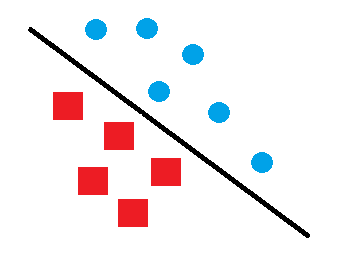
\includegraphics[width=0.3\textwidth]{imgs/Discriminativo.PNG}}
		\label{fig: Métodos de clasificación}
\end{figure}


Tras esto, se procede ha explicar distintos métodos de combinación existentes. Primero se hablara de bagging, explicando su funcionamiento y explicando con algún ejemplo su funcionamiento, para posteriormente hacer lo mismo con el boosting.

\subsection{Bagging}
Este método consiste en utilizar diferentes clasificadores en paralelo. Esto se hace ya que hay independencia entre los distintos clasificadores, por lo tanto los resultados que aporten uno no tendrá relación con la clasificación de otro, lo que permitirá reducir el error. 

Este método proviene de \textit{agregación de bootstrap}, algoritmo diseñado para mejorar estabilidad y precisión de los algoritmos. Su principal característica es reducir la varianza y evitar un sobreajuste en la clasificación. Para obtener la clasificación final se realiza una votación de los distintos métodos.

Como ejemplo de esta clasificación por votación, sería si tenemos 25 clasificadores iid (independientes e idénticamente distribuidas), cada uno con una tasa de error de 0.35, la probabilidad de que la mitad de clasificadores se equivoquen es de 0.06.

Cabe destacar que será mas sencillos tener clasificadores iid si cada uno de ellos se entrena con parámetros distintos.

\subsubsection{Random Forest}
Este método consiste en un \textit{bagging} de árboles binarios. Los árboles binarios son arboles cuyos nodos tendrán como máximo dos nodos descendientes, es decir, arboles de respuesta binaria. Cuando un nodo tiene solo un descendiente, este será el nodo hoja y se corresponderá a la clase del elemento de entrada.
El entrenamiento de este método consiste en dividir el conjunto de datos en dos recursivamente, hasta que queda todo dividido en clases. Lo normal es dividir en cortes paralelos a los ejes, pero en ocasiones se puede obviar esta restricción.

A continuación, en la imagen se observa lo contado de este método, como es gráficamente el árbol binario y la realización del entrenamiento con el conjunto de datos:


\begin{figure}[ht]
	\centering
		\subfloat[Estructura árbol binario.]{
   		\label{f:Estructura árbol binario.}
    	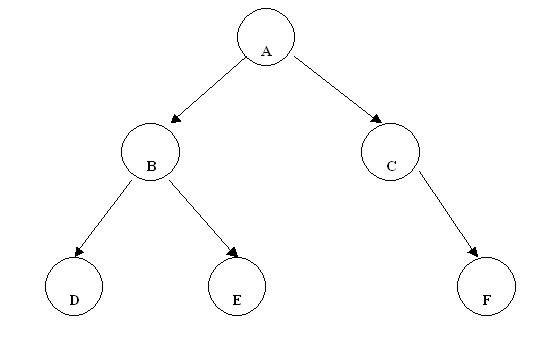
\includegraphics[width=0.5\textwidth]{imgs/arbolBinario.jpg}}
  		\subfloat[Entrenamiento para el arbol binario]{
  		\label{f:Entrenamiento para el arbol binario}
    	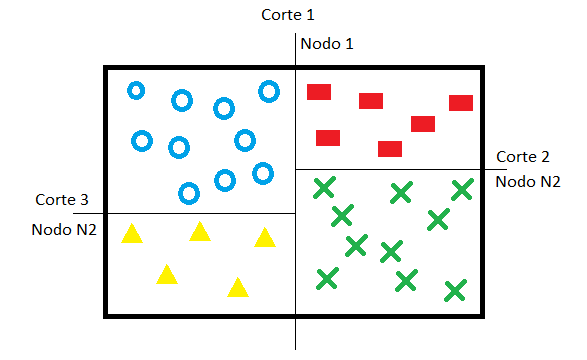
\includegraphics[width=0.5\textwidth]{imgs/DivisionNodos.PNG}}
		\label{fig: Árbol binario}
\end{figure}

Para saber si un corte es bueno, hay que mirar la entropía. Para ello, se parte de la distribución de datos original y se mira la distribución a cada lado del corte. Si hay mucho desorden (varias clases mezcladas a cada lado) o queda ordenado. 

La ventaja de este método es que es rápido y sencillo de realizar.

La desventaja principal, es muy complicado llegar a un árbol que clasifique todo correctamente con los datos del entrenamiento. Si se da este caso, probablemente este ocurriendo \textit{sobreaprendizaje}.

A continuación se observan diferentes imágenes. En la primera de ellas se da el desajuste, que se da cuando no se encuentran los patrones que clasifican correctamente las clases. En la segunda se da el clasificador apropiado para el conjunto de datos dado. Por último, en la tercera imagen se muestra el sobreajuste, es decir, que se clasifica a partir de los datos del conjunto en lugar de con los patrones que las clases ofrecen.


\begin{figure}[ht]
	\centering
		\subfloat[Desajuste.]{
   		\label{f:Desajuste del clasificador.}
    	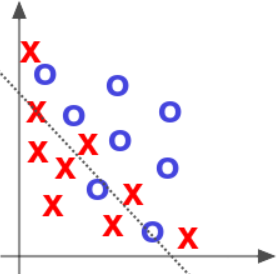
\includegraphics[width=0.3\textwidth]{imgs/desajuste.PNG}}
  		\subfloat[Clasificador óptimo]{
  		\label{f:Clasificador óptimo}
    	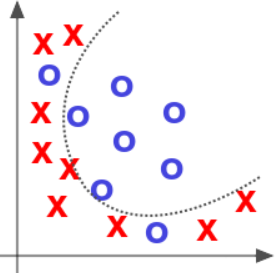
\includegraphics[width=0.3\textwidth]{imgs/optimo.PNG}}
    	\subfloat[Sobreajuste del clasificador]{
  		\label{f:Sobreajuste del clasificador}
    	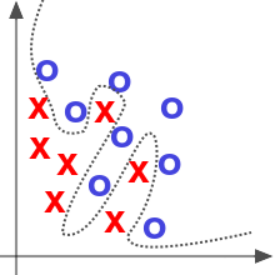
\includegraphics[width=0.3\textwidth]{imgs/sobreajuste.PNG}}
		\label{fig: Distintas clasificacioens del arbol binario}
\end{figure}


Para evitar ese sobreajuste, se utiliza \textbf{bagging} de arboles binarios, obteniendo así la técnica \textbf{Random Forest}. 

Este método consiste en generar diversas muestras (inyectando aleatoriedad), entrenar diferentes arboles y realizar la votación por mayoría para la clasificación de un elemento. 

Las características principales de este método son:
\begin{itemize}
  \item \textbf{Paralelismo: }Permite el entrenamiento y ejecución de los distintos arboles en paralelo. Dichos arboles son arboles independientes.
  \item \textbf{Reducción de la varianza: }Como de diferentes serán las predicciones de un modelo si se toman muestras distintas del mismo conjunto de datos.
  \item \textbf{Reducción del sesgo: }Diferencia en promedio existente entre los valores obtenidos y los valores reales.
\end{itemize}

Otros parámetros relacionados con este método son:
\begin{itemize}
  \item \textbf{Número de árboles: } Utilizando varios arboles se consigue minimizar el error, pero utilizar demasiados arboles puede ser innecesario.
  \item \textbf{Número máximo de niveles: } Cada árbol tendrá un número determinado de niveles. Cuanto más niveles, existirá una mayor precisión, pero evitando llegar al sobreajuste previamente comentado.
\end{itemize}




\subsection{Boosting}
El \textit{boosting} consiste en la creación de un clasificador fuerte combinando varios clasificadores básicos. Cuando se combinan diferentes clasificaciones, cada uno contribuye según su peso, el cual se asigna en función de la exactitud en sus predicciones. 

La idea principal de este método es que ningún clasificador ofrece siempre el mejor resultado que la combinación de todos los clasificadores, ya que esto va a suavizar los errores de cada uno, obteniendo un clasificador mas eficiente. 

Como principales características de este método, hay que destacar:
\begin{itemize}
  \item Los clasificadores se construyen secuencialmente. cada clasificador se construye con información del clasificador previo.
  \item Se realiza un muestreo selectivo para el conjunto de datos de entrenamiento.
  \item Es mas probable que se seleccione un elemento mal clasificado para el entrenamiento del siguiente clasificador.
\end{itemize}


El procedimiento original de boosting se basa en realizar los siguientes pasos:

\begin{enumerate}
\item Extraer un subconjunto de la muestra de aprendizaje y entrenar un primer clasificador con el. 
\item Extraer otro subconjunto de la muestra de aprendizaje y añadir la mitad de las muestras mal clasificadas anteriormente. Con esto se entrena un segundo clasificador. 
\item Encontrar un subconjunto de muestras con los cuales los clasificadores previamente entrenados retornen resultados diferentes y utilizar este subconjunto para entrenar un tercer clasificador.
\item Combinar los tres clasificadores realizando una votación por mayoría. 
\end{enumerate}

A continuación, se procede a hablar del algoritmo mas utilizado de boosting, llamado adaboost, y fue el primero de este tipo que consiguió resultados óptimos.

\subsubsection{AdaBoost}
Su nombre proviene de \textit{Adaptative Boosting} y consiste, como se ha explicado previamente, en conseguir un clasificador fuerte a partir de clasificadores débiles. Para ello, este método utiliza el siguiente procedimiento:

\begin{enumerate}
\item Se inicializan los pesos para cada observación de la muestra, teniendo inicialmente todas las muestras el mismo peso:

$$w_i =\frac{1}{N} ,  i = 1,2,..., N.$ 

\item Para m = 1, 2, ..., M

\begin{enumerate}
\item Entrenar el clasificador básico
\item Estimar el error $G_m (x)$
\item Clasificar la importancia del error. Hay que tener en cuenta las observaciones previas:

$$err_m = \frac{\sum_{i=1}^{n}w_i I(y_i \neq G(x_i))}{\sum_{i=1}^{n}w_i}$

\item Establecer nuevos pesos(si clasifica bien, se asigna un peso bajo, en caso contrario se asignará un peso alto).

$$ \alpha_m = \log {(\frac{1 - err_m}{err_m})} $

\item Actualizar los pesos.

$$ w_i = w_i e^{\alpha_m I(y_i \neq G(x_i))} $


\end{enumerate}

\item Retornar el clasificador final:

$$ G(x) = sign(\sum_{m=1}^{M}\alpha_m G_m(x))  $


\end{enumerate}

Por todo esto, suponiendo que $err_m < 0.5 $, cuando $\alpha_m \geq 0$, en cada iteración aumentan el peso las observaciones mal clasificadas, mientras que lo disminuyen las bien clasificadas.

Las siguientes imágenes corresponden a un ejemplo de este clasificador:

\begin{figure}[ht]
	\centering
		\subfloat[Conjunto de datos.]{
   		\label{f:Conjunto de datos 1.}
    	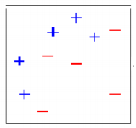
\includegraphics[width=0.23\textwidth]{imgs/Adaboost1.PNG}}
		\subfloat[Clasificador 1.]{
   		\label{f:Clasificador 1.}
    	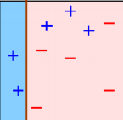
\includegraphics[width=0.23\textwidth]{imgs/Adaboost2.PNG}}
  		\subfloat[Clasificador 2.]{
  		\label{f:Clasificador 2.}
    	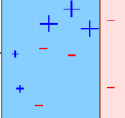
\includegraphics[width=0.23 \textwidth]{imgs/Adaboost3.PNG}}
    	\subfloat[Clasificador 3.]{
  		\label{Clasificador 3.}
    	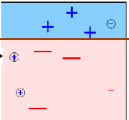
\includegraphics[width=0.23\textwidth]{imgs/Adaboost4.PNG}}
		\label{fig: Clasificadores Adaboost.}
\end{figure}


El primer clasificador intenta separar positivos y negativos, cometiendo 3 errores. El peso de estas muestras incrementa para el siguiente clasificador, mientras que el peso de las otras muestras disminuye.
En el siguiente clasificador, las muestras previamente mal clasificadas ahora se clasifican correctamente, pero 3 de los datos negativos ahora se clasifican mal, por lo que suben su peso. 
En el último clasificador, los últimos negativos mal clasificados se clasifican de forma correcta debido al aumento de su peso, mientras que otro de los negativos se clasifica de forma incorrecta.

Con todo esto, el clasificador final formado por el conjunto de los tres clasificadores quedaría de la siguiente manera:
\begin{figure}[ht]
	\centering
		\subfloat[Clasificador final.]{
   		\label{f:Clasificador final.}
    	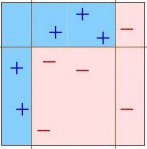
\includegraphics[width=0.3\textwidth]{imgs/AdaboostFinal.PNG}}
		\label{fig: Clasificador final Adaboost.}
\end{figure}

Obteniendo así un clasificador mejor que los tres vistos previamente por separado.


\subsubsection{SAMME}
Se trata de otro método de boosting, el cual sigue un proceso parecido al clasificador previamente explicado pero con algunas variaciones, como se cuenta a continuación:


\begin{enumerate}
\item Los pesos en la inicialización se obtienen de igual forma:

$$ w_i =\frac{1}{N} ,  i = 1,2,..., N.$ 

\item Para m = 1, 2, ..., M
\begin{enumerate}
\item Se obtiene el clasificador que minimice $\epsilon_m $ (error ponderado):

$$ \epsilon_m = \sum_{y_i \neq C_m(x_i)} w_i $

\item Calcular:

$$ \alpha_m = 1/2 \log{\func{1 - \epsilon_m}{\epsilon_m}} + \ln(K-1) $

Siendo K el número de clases.

\item Actualizar los pesos:

$$ w_i = w_i e^{\alpha_m (x)I(y_i \neq C_m(x_i))} $


\item Escalar pesos para que sumen 1:

$$ w_i = \func{w_i}{\sum_{j=1}^{n} w_j} $

\end{enumerate}

\item Siendo el clasificador final:

$$ C(x) = \arg\underset{j\epsilonY}\max \sum_{m = 1}^{M} \alpha_m I (C_m(x) = j) 	Y = {1,...,K} clases.  $ 

\end{enumerate}

Una vez explicado el contexto mas general sobre el que se basa el trabajo, se continua explicando el entorno mas cercano de este trabajo. 


\section{BAdaCost}
El algoritmo sobre el que se trabaja en este trabajo es BAdaCost, el 
cual se define como un algoritmo de clasificación sensible al costo de varias clases.
Para la realización de este algoritmo, se utiliza un conjunto de clasificadores débiles multi-clase sensible a los costes para obtener una regla de clasificación basada en boosting. Para poder explicar este algoritmo, primero hay que hablar sobre CMEL \textit{Cost-sensitive Multi-class Exponential Loss}, algoritmo que optimiza la perdida en varios algoritmos de clasificación como AdaBoost, SAMME, Cost-sensitive AdaBoost o PIBoost. BAdaCost consigue importantes mejoras de rendimiento en comparación con los algoritmos anteriores.

Este algoritmo busca minimizar la pérdida de CMEL, $ \sum_{n=1}^{N} L_c (l_c, f(x_n)) $ siendo ${{(x_n, l_n)}}$ los datos de entrenamiento. Siendo un algoritmo de Boosting, la minimización se realiza mediante un modelo aditivo por etapas, $f(x) = \sum_{m=1}^{M} \beta_m g_m$. El clasificador seleccionado trata de optimizar $\beta_m$ en cada iteración a lo largo de $g_m$. Para calcular esto se siguen los siguientes pasos:

Búsqueda de ($\beta_m$,$g_m(x)$) óptimos para CMEL. Siendo C la matriz de costes de un problema multiclase:

$$ (\beta_m, g_m(x) = \arg\underset{\beta, g}\min \sum_{n=1}^{N} exp(C^{*}(ln, -)(f_m-1 (x_n) + \beta_g(x_n)) $

es la misma solución para:

$$ (\beta_m, g_m(x)) = \arg\underset{\beta, g}\min \sum_{n=1}^{N} S_j exp(\beta C^{*}(j,j)) + \sum_{j=1}^{K} \sum_{k\neq j} E_j,k exp ((\beta C^{*}(j,j))$

Donde $S_j = \sum_{{n:g(x_n)=l_n=j}} w(n)$, $E_{j,k} = \sum_{{n:g(x_n)=l_n=j}}$ y el peso de la instancia de entrenamiento n es:

$$ w(n) = exp{(C^{*}(ln,-)\sum_{t=1}^{m-1}\beta_m f_m (x_n))} $

Dada una dirección conocida de g, el $\beta$ óptimo se puede obtener como solución de:

$$ \sum_{j=1}^{K} \sum_{k \neq j} E_{j,k} C(j,k) A(j,k)^{\beta} = \sum_{j=1}^{K} \sum_{h = 1} S_j C(j,h) A(j,j)^{\beta}$

siendo $ A(j,k) = exp(C^{*}(j,k)) ∀ j,k \epsilon L$. Por último, dado un $\beta$ conocido, la dirección descendiente óptima g, equivalente a G, es dada por:

$$ \arg\underset{G}\min \sum_{n=1}^{N}w(n) A(l_n,l_n)^{\beta}I(G(x_n) = l_n) + \sum_{n=1}^{N} w_n \sum_{k \neq l_n} A(l_n,k)^{\beta} I (G(x_n) = K) $

El código de ejecución de este método se puede explicar como:

\begin{enumerate}
\item Se inicializan los pesos para cada observación de la muestra, teniendo inicialmente todas las muestras el mismo peso:

$$w_i =\frac{1}{N} ,  i = 1,2,..., N.$ 

\item Se calculan las matrices $C^{*}$ y A para C.

\item Para m = 1, 2, ..., M
\begin{enumerate}
\item Se obtiene $G_m$ para $\beta = 1$

\item Se traduce $G_m$ en $g_m$

\item Se calculan $E_{j,k}$ y $S_j$ para todo j,k.

\item Se calcula $\beta_m$

\item $w(n) = w(n) exp (\beta_m C^{*}(ln,-)g_m(x_n))$

\item Se normaliza el vector w

\end{enumerate}

\item Se obtiene la salida $ H(x) = \arg\min_k C^{*}(k,-)(\sum_{m=1}^{M} \beta_m g_m(x))$

\end{enumerate}

A continuación, se muestra una tabla de costes promedio y desviación estandar de distintos algoritmos de clasificación, comparando BAdaCost con Ada.C2M1, MultiBoost y Lp-CSB. Se puede observar como en general se obtienen mejores resultados:

\begin{figure}[ht]
	\centering
		\subfloat[Tabla comparativa.]{
   		\label{f:Tabla comparativa.}
    	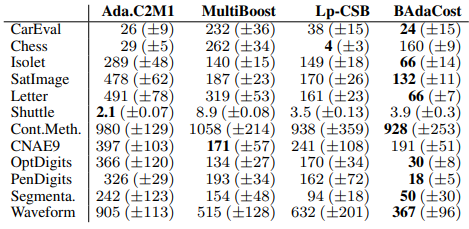
\includegraphics[width=0.15\textwidth]{imgs/TablaComparativa.PNG}}
\end{figure}



Tras haber una breve introducción, se va a explicar lo realizado en este proyecto. En el capítulo 2 se habla sobre los objetivos propuestos y la metodología utilizada para llegar a ellos. Tras ello, en el capítulo tres se va a hablar sobre el algoritmo realizado, la implementación del diseño y el código realizado. Después, en el capítulo 4 se van a comentar los experimentos realizados y los resultados obtenidos. Finalmente, en el capítulo 5 se explicaran las conclusiones obtenidas y los próximos trabajos a realizar.































\lhead[]{CAPÍTULO \thechapter. OBJETIVOS}
\chapter{Objetivos}\label{cap.Objetivos}
Una vez presentado el contexto de este TFM en el primer capítulo, yendo de lo más general (tipos de clasificadores) a lo más cercano (el clasificador a utilizar), en este capítulo se van a explicar los objetivos concretos a conseguir y la metodología utilizada para llegar a ello.

\section{Objetivo principal}
El objetivo principal es hacer funcionar BAdaCost detector, desarrollado para matlab, en C++. Para ello, utilizando la misma imagen de entrada y el mismo detector, hay que obtener la misma salida (mismas detecciones o muy parecidas). Para llegar a esto, se han propuesto distintas fases:

\begin{itemize}
\item \textbf{Extracción de características: } Para poder clasificar bien los elementos de las imágenes, hay que extraer de forma correcta las características. En este caso los detectores trabajan con diferentes características (espacios de color, magnitud del gradiente y magnitud del histograma). Por ello, se realiza el desarrollo para C++, comparando siempre que los resultados obtenidos sean los mismos que en Matlab.

\item \textbf{Procesamiento de las características: } Una vez se realiza la extracción de características, pueden darse distintos procesos de transformación como redimensionados, suavizados o relleno (padding) sobre lo obtenido. El siguiente paso era asegurar que estos procesos retornan también el mismo resultado en C++ que en Matlab.

\item \textbf{Realizar la detección: } Una vez se tienen las características procesadas igual que en Matlab, lo siguiente es realizar la detección. Para ello, hay que guardar el detector de Matlab en un formato legible en C++, leer los parámetros del detector y poder utilizarlos correctamente. Una vez se pueden cargar los parámetros del detector, desarrollar el algoritmo de detección en C++.
\end{itemize}


\section{Requisitos}
Para la realizaci\'on de los objetivos anteriormente citados, se tiene que conseguir una soluci\'on que cumpla las siguientes caracter\'isticas:
\begin{itemize}
\item Que se trate de un algoritmo robusto, capaz de trabajar con distintos clasificadores y que no dependa de unos parámetros determinados, sino que sea capaz de obtener resultados óptimos en distintos casos.

\item Que el algoritmo sea capaz de trabajar en distintos tipos de máquinas, no necesitando unas características específicas, solo que permita ejecutar C++ y tenga la librería OpenCV instalada.

\end{itemize}

\section{Metodolog\'ia}

La metodología propuesta es un desarrollo en espiral. Para ello se proponen semanalmente reuniones con el tutor, en las cuales se presentaba lo conseguido en el último periodo en relación a los objetivos propuestos y se proponían los nuevos objetivos para la siguiente reunión. Sobre las tareas propuestas se evaluaban los riesgos que podían darse y los avances que se conseguirían en función del camino tomado. Después, se continuaba desarrollando el algoritmo para conseguir los objetivos.Se probaba en todo momento mediante tests si lo desarrollado funcionaba o no. En función del resultado de estos tests, se determinaba si el objetivo se había conseguido o no. Si no se conseguía, analizar el fallo para solventarlo. En caso de que se consiguiese o estar cerca, se proponían nuevos objetivos para continuar con el trabajo.

\begin{figure}[H]
	\centering
		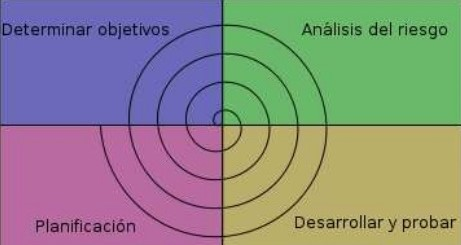
\includegraphics{imgs/metodologia-espiral.jpg}
        \caption{M\'etodo de desarrollo en espiral}
	\label{fig:Desarrollo en espiral}
\end{figure}

Durante todo el desarrollo, se utilizado GitHub como repositorio del código, explicando cuales eran los últimos avances subidos en los \textit{commits} y generando un \textit{issue} por cada tarea a realizar, poniendo en él las diferentes dudas que surgían e indicando la resolución final. De esta forma, se conseguía un desarrollo y una comunicación fluida, quedando el código públicamente accesible en \href{https://github.com/RoboticsURJC-students/2017-tfm-jorge_vela}{https://github.com/RoboticsURJC-students/2017-tfm-jorge_ vela}.



\section{Plan de trabajo}
La planificación seguida en el desarrollo ha incluido las siguientes fases:

\begin{itemize}
\item{Investigación: }Comprender el funcionamiento del \textit{toolbox} de badacost, ver la organización del código y su funcionamiento, tanto de las funciones por separado como el algoritmo en conjunto, para ver la extracción de características y el funcionamiento del conjunto final.

\item{Desarrollo del código: } Una vez visto el funcionamiento, trabajar en el código para que BAdaCost funcionara en C++ de forma robusta. Para ello, por cada clase o función que se creaba, se realizaba un test de prueba. Con esto, cuando se obtiene el resultado de C++ se compara con el de Matlab, de forma que se asegura un resultado correcto. Los tests también ayudan si a lo largo del desarrollo, se produce algún cambio en el código. Al comprobar continuamente que todo lo anterior funciona, si un cambio provoca fallo es muy fácil de detectar y saber porque ocurre.

\item{Compatibilidad entre Matlab y C++: } Bien sea para comparar los datos, o para utilizar el mismo detector, tiene que haber un método que permita tener datos iguales en ambos lenguajes. Para ello se ha utilizado el formato YML. Con esto, se pueden guardar todo tipo de datos desde matlab (como el resultado de funciones determinadas o los parámetros de un detector) y leerlo desde C++.
En Matlab se ha creado una función que guarda lo deseado con un formato determinado, el cual se lee desde el código desarrollado en C++.  

\end{itemize}































\lhead[]{CAPÍTULO \thechapter. ALGORITMO}
\chapter{Algoritmo BAdaCost en C++}\label{cap.algoritmo} 
En este capítulo se describe el algoritmo a través del cual se ha llegado a la solución de lo planteado en los objetivos.

Este algoritmo tiene que permitir la detección de distintos elementos utilizando el clasificador BAdaCost. Para ello, en este capítulo primero se explica el diseño y organización del código. Tras ello, se explica como se ha desarrollado cada clase y función y los resultados obtenidos por cada una. Finalmente explicar el detector obtenido, el cual utiliza todo lo desarrollado previamente, retornando si en la imagen de entrada se encuentra el elemento de interés y donde está situado.

\section{Estructura del código.}

Para la realización de este algoritmo, se ha seguido un a estructura que, siguiendo una estructura de lo mas general a lo mas específico, se puede resumir de la siguiente forma:

\begin{itemize}

\item \textbf{BadacostDetector: } Clase del detector que se utiliza en este proyecto. Para su funcionamiento, contiene una función la cual requiere como parámetro una imagen de entrada y un fichero que contenga los parámetros del clasificador. Como salida retorna un vector con las distintas detecciones en un formato especifico.

\item \textbf{ChannelsPyramid: } Encargada de calcular la pirámide de características a partir de la imagen de entrada. Para ello, calcula los distintos tamaños que tiene que tener la imagen en función de los parámetros de entrada y llama al calculo de estas características para los distintos tamaños.

\item \textbf{ChannelsExtractorLDCF: } A partir de una imagen de entrada, extrae las características de la imagen, obteniendo imágenes (cv::Mat) como resultados, y realiza una convolución con filtros cargados en el detector.

\item \textbf{ChannelsExtarctorACF: } Calcula las características de la imagen de entrada (canales de color en LUV, magnitud del gradiente y características HOG) retornando cada característica en un cv::Mat.

\item \textbf{ChannelsExtractorGradMag: } Calcula la magnitud del gradiente y la orientación por cada píxel de la imagen.

\item \textbf{ChannelsExtractorGradHist: } Calcula el histograma de gradiente orientado. Para cada región de tamaño determinado, calcula un histograma de gradientes, con cada gradiente cuantificado por su ángulo y ponderado por su magnitud.

\item \textbf{ChannelsExtractorGradLUV: } Dada una imagen de entrada RGB retorna un vector con los canales de color L, U, V. 

\item \textbf{Utils: } Contiene diferentes funciones que utilizan las clases previamente explicadas.

\end{itemize}

Una vez hecha una introducción al algoritmo, habiendo definido cada una de las partes, se pasa a redactar cada una de las clases y funciones desarrolladas:























\lhead[]{CAPÍTULO \thechapter. EXPERIMENTOS}
\chapter{Experimentos}\label{cap.experimentos}

\lhead[]{CAPÍTULO \thechapter. Conclusiones}
\chapter{Conclusiones}\label{cap.conclusiones}


\section{L\'ineas futuras}




\end{document}
